\section{Augmentation}
\label{sec:augment}

We present an approach for augmenting ContraPro to improve \textsc{cr}.    
%
Augmentation systematically expands the data to improve a model's robustness~\citep{kafle2017data}.
%
While challenging for \textsc{nlp},  we focus on a narrow problem which lends itself to easier data manipulation. 
%
Figure~\ref{fig:templates} shows that our model is capable of modeling the gender of nouns.
%
However, they also show a strong  prior for translating \textit{it} to \textit{es} and very little \coref{} capability.
%
Our goal with the augmentation is to alter the prior and test if this can improve \coref{} in the model.


We augment our training data 
and call it Antecedent-free augmentation (\textsc{afa}).
%
We identify candidates for augmentation as sentences where a coreferential \textit{it} refers to an antecedent not present in the current or previous sentence  (e.g., \textit{I told you before. $<$SEP$>$ \underline{It} is red.} $\rightarrow$ \textit{Ich habe dir schonmal gesagt. $<$SEP$>$ \underline{Es} ist rot.}).
%
We create augmentations by adding two new training examples where the gender of the German translation of ``it'' is modified 
(e.g., the two new targets are ``\textit{Ich habe dir schonmal gesagt. $<$SEP$>$ \underline{Er} ist rot.}'' and ``\textit{Ich habe dir schonmal gesagt. $<$SEP$>$ \underline{Sie} ist rot.}'').
The source side remains the same.
%
Table~\ref{table:manual-examples-augmentations-main} provides an additional example.
%
Antecedents and coreferential pronouns are identified using a \coref{} tool \citep{clark2016deep,clark-manning-2016-improving}.
%
We fine-tune our  already trained concatenation
model on a dataset consisting of the candidates and the augmented samples. 
%
As a baseline, we fine-tune on the candidates to confidently say that any potential improvements come from the augmentations. 


\subsection{Results}
Results for adversarial attacks on ContraPro and on our templates are independent and are discussed separately.  

\begin{figure}[ht!]
	\centering
	\includegraphics[width = \linewidth]{\figfile{F3.pdf}}
	\caption{Results comparing unaugmented and augmented \textsc{concat} on ContraPro and same 3 attacks as in Figure~\ref{fig:contrapro}. Results with non-augmented \textsc{concat} are the same as Figure \ref{fig:contrapro}.}
	\label{fig:augmentation-contrapro}
\end{figure}

\subsubsection{Adversarial Attacks}

\textsc{afa} provides large improvements, scoring 85.3\% on ContraPro (Figure~\ref{fig:augmentation-contrapro}).
%
The \textsc{afa} baseline  (fine-tuning on the augmentation candidates only) improves by 1.94\%, presumably because many candidates consist of coreference chains of ``it'' and the model learns they are important for coreferential pronouns. However, the improvement is small compared to \textsc{afa}. 
% translation. 



Prediction accuracy on \textit{er} and \textit{sie} is substantially increased, suggesting that the augmentation removes the strong bias towards \textit{es}. %Templates provide further evidence about this. 
%
Although, the adversarial attacks lower \textsc{afa} scores, 
in contrast to \textsc{concat}, the model is more robust and the accuracy degradation is substantially lower (except on the synonym attack).
% 
We experiment with different learning rates during fine-tuning and 
present results with the \textsc{lr} that obtain 
the  best  baseline ContraPro score.
%
Furthermore, \textsc{concat}  and \textsc{afa} obtain $31.5$  and $32.2$ \textsc{BLEU} on ContraPro, showing that this fine-tuning procedure, which is tailored to pronoun translation, does not lead to any degradation in overall translation quality.

\subsubsection{Templates}



The prior over gender pronouns is more evenly spread and not concentrated on \textit{es}.
%
This provides for a more even distribution on the Position and Role Prior template.

The augmented model has higher accuracy on markable detection, improving by $27.6\%$. 
%
Results for  the templates are in Figure~\ref{fig:augmentation-templates}.




\begin{figure}[!h]
	\centering
	\includegraphics[width = \linewidth]{\figfile{F4.pdf}}
	
	\begin{comment}
	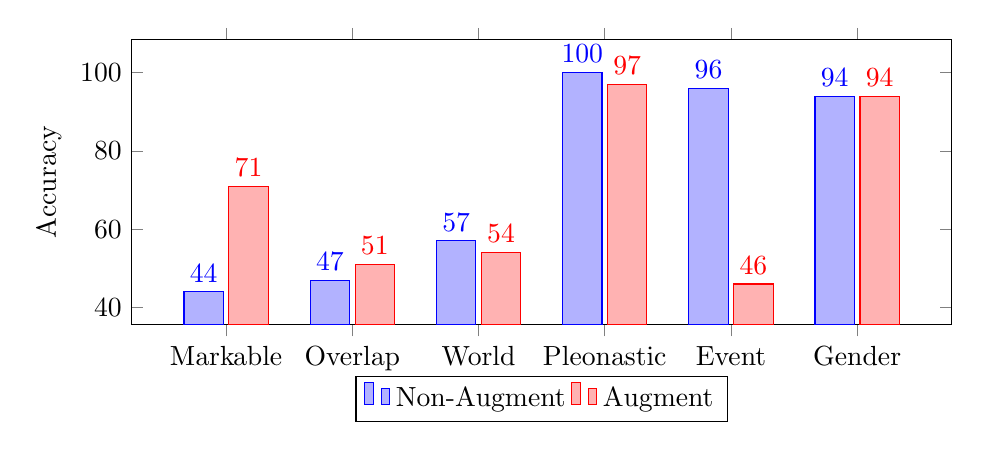
\begin{tikzpicture}
	\begin{axis}[
	ybar,
	enlargelimits=0.15,
	legend style={at={(0.5,-0.18)},
	anchor=north,legend columns=-1},
	ylabel={Accuracy},
	symbolic x coords={Markable,Overlap,World,Pleonastic,Event,Gender},
	xtick=data,
	nodes near coords,
	nodes near coords align={vertical},
	height=5.2cm,
	width=12cm,
	bar width=0.5cm,
	]
	\addplot coordinates {(Markable,44) (Overlap,47) (World,57) (Pleonastic,100) (Event,96) (Gender,94)};
	\addplot coordinates {(Markable,71) (Overlap,51) (World,54) (Pleonastic,97) (Event,46) (Gender,94)};
	\legend{Non-Augment,Augment}
	\end{axis}
	\end{tikzpicture}
	\end{comment}
	% \caption{Augmentation improves \textsc{Concat}'s pronoun translations on ContraCAT.  We speculate that this is explained by a readjusting of the prior. }
	\caption{ContraCAT results with unaugmented and augmented \textsc{concat}. We speculate that readjusting the prior over genders in augmented \textsc{concat} explains the improvements on Markable and Overlap.}
	\label{fig:augmentation-templates}
\end{figure}

% Considering our augmentation approach, 
No improvements are observed on the World Knowledge template.
Pleonastic cases are still accurate, although not perfect as with \textsc{concat}. 
% The shift in prior distribution over pronouns causes a small number of mistakes. 
The Event template identifies a systematic issue with our augmentation. We presume this is due to the \coref{} tool marking cases where \textit{it} refers to events. 
%
We do not  apply any filtering and augment these cases as well,
thus creating wrong examples (an event reference \textit{it} cannot be translated to \textit{er} or \textit{sie}). 
%
As a result, the scores are significantly lower compared to \textsc{concat}. 
%
This issue with our model is not visible on ContraPro and the adversarial attacks results. In contrast, the Event template easily identifies this problem.

\textsc{afa} has a similar accuracy to the unaugmented baseline on the Gender template. 
%
However,
despite increasing by 3.8\%, results on Overlap are still underwhelming. 
%
Our analysis shows that augmentation helps in changing the prior. 
%
We believe this provides for improved \coref{} heuristics which in turn provide for an improvement in coreferential pronoun translation. 
%
Nevertheless, the Overlap template shows that augmented models still do not solve \coref{} in a fundamental way.

